\subsection{V2}
Video \textit{V2} is recorded at 29 fps. Only cars driving from the left to the right are detected and tracked. In this
experiments
frames 83-109 of
video \textit{V2} are
shown.
\subsection{V2 -- GM-PHD with constant detection probability}
The measurements for GM-PHD filter with constant detection probability are obtained by the YOLO object detection
model. The parameters' values are displayed in Table \ref{tab:E1-V2-S0}.
\begin{table}[!h]
    \centering
    \begin{tabular}{|c|c|c|c|c|c|}
        \hline
        $P_{D}$ & $P$ & $\sigma_{\upsilon}$ & $\sigma_{\epsilon}$ & $T_p$ & $T_{YOLO}$ \\ \noalign{\hrule height 1.5pt}
        0.9 & $diag(100,100,100,100)$ & 0.1 & 30 & 0.1 & 0.3\\
        \hline
    \end{tabular}
    \caption{The parameter settings for the experiment E1-V2 with the constant detection probability.}
    \label{tab:E1-V2-S0}
\end{table}

Figure \ref{fig:E1-V2-S0} display the performance the the GM-PHD filter with the constant detection probability.
\begin{itemize}
    \item \textbf{\ref{fig:E1-V2-S0:01}:} The sequence starts with the frame no. 83. At this time, four targets are
    already initialized and successfully detected.
    \item \textbf{\ref{fig:E1-V2-S0:02}:} The objects are small compared to the whole size of frame. This size
    difference causes the filter, that targets in close neighbourhood shares measurements and more targets appear in
    the scene.
    \item \textbf{\ref{fig:E1-V2-S0:03}:} The fourth car is not detect by the YOLO model, but the target survives.
    \item \textbf{\ref{fig:E1-V2-S0:04}:} The previously undetected car is detected again and the target is still
    tracked. Another car approaches the spawning point.
    \item \textbf{\ref{fig:E1-V2-S0:05}:} The car in spawning area is not detected and probably its weight was too
    low to survive. The first car exits the scene.
    \item \textbf{\ref{fig:E1-V2-S0:06}:} The car at the spawning point is detected again and still close enough to
    be initialized as a target. The scene ends with four true objects and four right targets.
\end{itemize}


The GM-PHD filter with constant detection probability is accurate in scenarios, where the object detector does not
miss detections at a higher rate. Graph \ref{gr:E1-V2-S0} shows that the number of displayed targets is close enough
to the true count. Even false detections created by YOLO does not mislead the filter.


\begin{figure}[H]
    \centering
    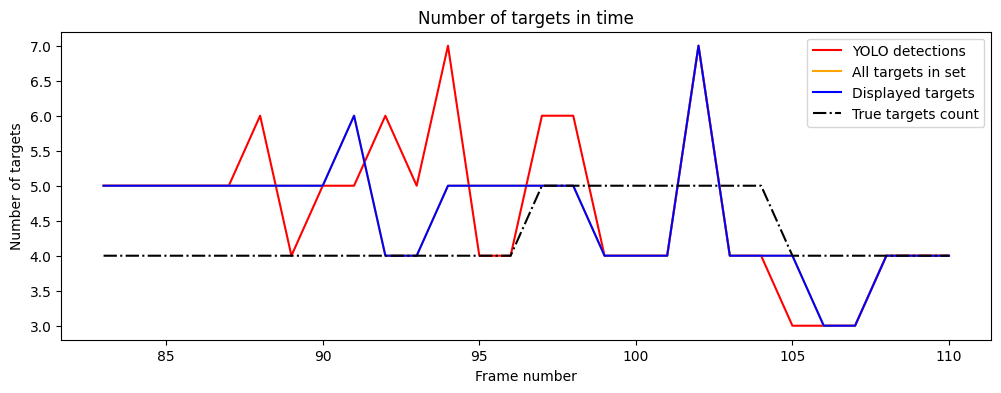
\includegraphics[width=\linewidth]{../../../experiments/E1/V2/noPd/staticPd_det}
    \caption{Development chart of the number of detected targets, targets in filter's queue, displayed targets and true
    targets' count.}
    \label{gr:E1-V2-S0}
\end{figure}

\begin{figure}[H]
    \centering
    \begin{subfigure}{0.48\textwidth}
        \centering
        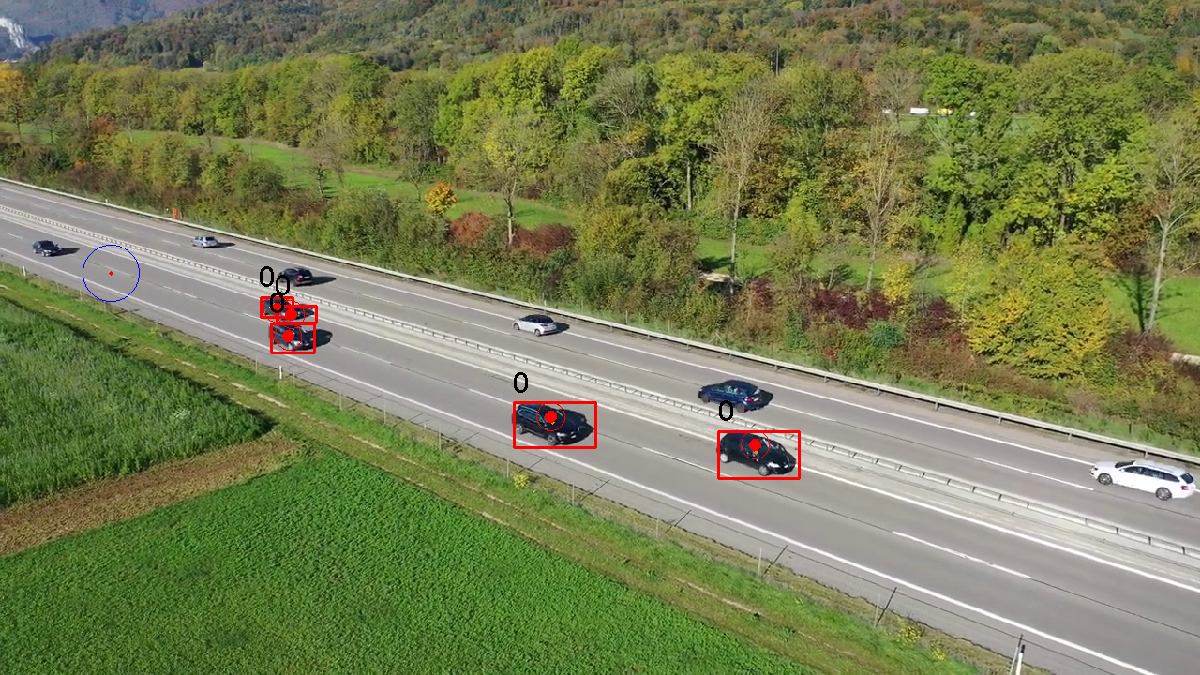
\includegraphics[width=\linewidth]{../../../experiments/E1/V2/noPd/83}
        \caption{Frame number: 83.}
        \label{fig:E1-V2-S0:01}
    \end{subfigure}
    \begin{subfigure}{0.48\textwidth}
        \centering
        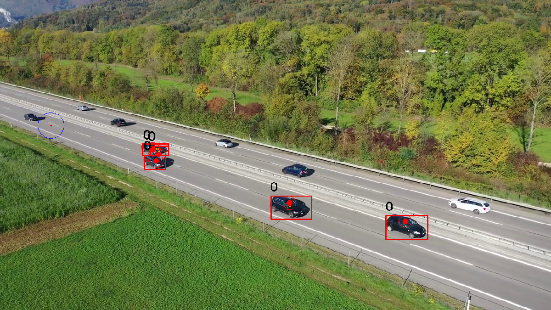
\includegraphics[width=\linewidth]{../../../experiments/E1/V2/noPd/90}
        \caption{Frame number: 90.}
        \label{fig:E1-V2-S0:02}
    \end{subfigure}
    \\
    \begin{subfigure}{0.48\textwidth}
        \centering
        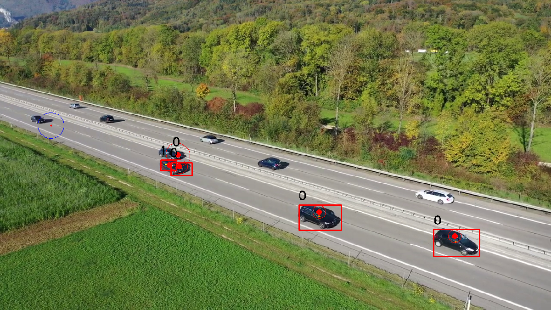
\includegraphics[width=\linewidth]{../../../experiments/E1/V2/noPd/95}
        \caption{Frame number: 95.}
        \label{fig:E1-V2-S0:03}
    \end{subfigure}
    \begin{subfigure}{0.48\textwidth}
        \centering
        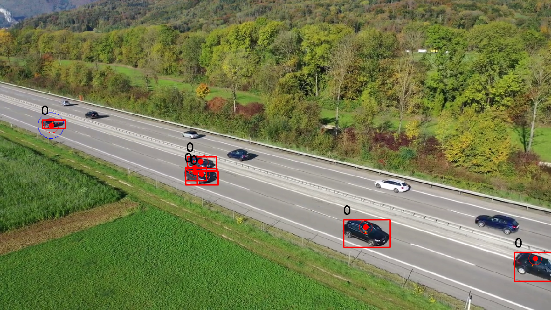
\includegraphics[width=\linewidth]{../../../experiments/E1/V2/noPd/102}
        \caption{Frame number: 102.}
        \label{fig:E1-V2-S0:04}
    \end{subfigure}
    \\
    \begin{subfigure}{0.48\textwidth}
        \centering
        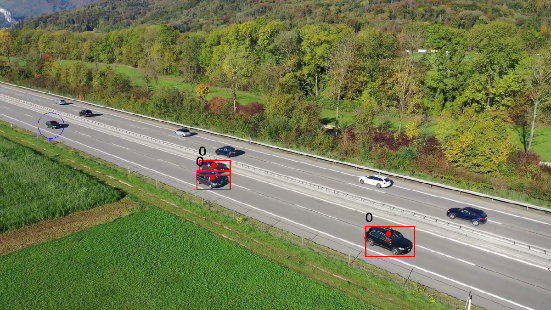
\includegraphics[width=\linewidth]{../../../experiments/E1/V2/noPd/105}
        \caption{Frame number: 105.}
        \label{fig:E1-V2-S0:05}
    \end{subfigure}
    \begin{subfigure}{0.48\textwidth}
        \centering
        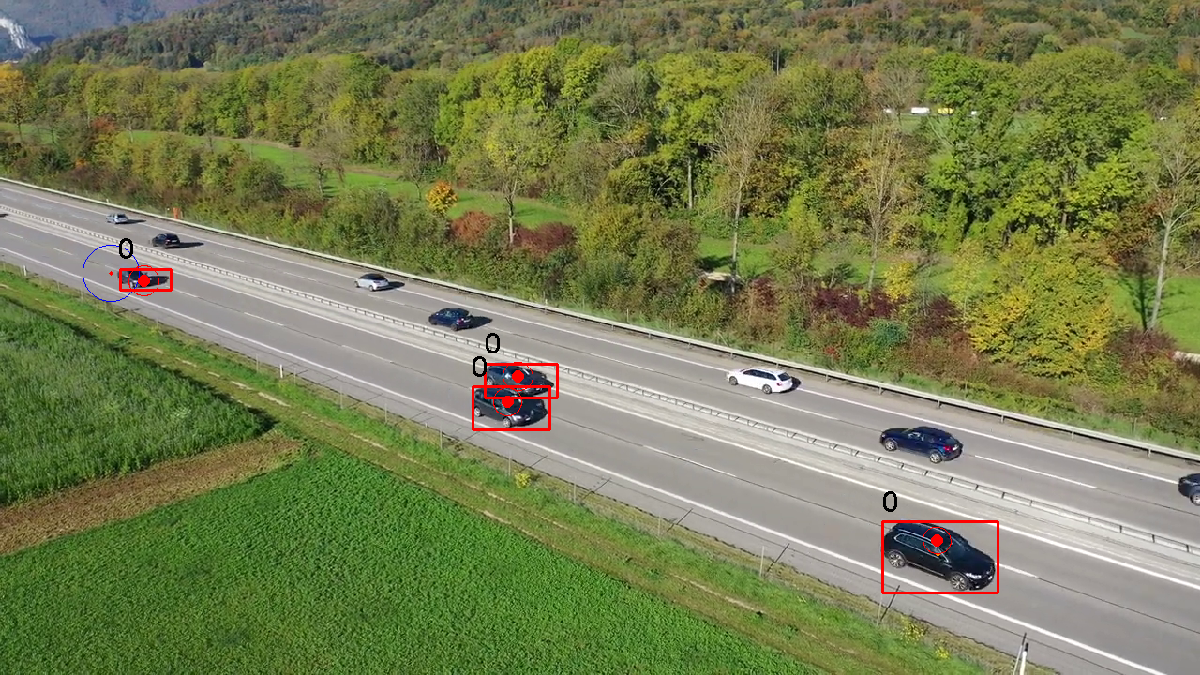
\includegraphics[width=\linewidth]{../../../experiments/E1/V2/noPd/110}
        \caption{Frame number: 110.}
        \label{fig:E1-V2-S0:06}
    \end{subfigure}
    \caption{Image sequence of tracked objects using GM-PHD filter with constant detection probability.}
    \label{fig:E1-V2-S0}
\end{figure}


\subsection{V2 -- GM-PHD with dynamic detection probability}
Experiments on video \textit{V2} using GM-PHD filter with dynamic detection probability and different settings are
demonstrated in following sections.
\subsubsection{S1 -- YOLO + YOLO}
This experiment uses settings \textit{S1}, where the YOLO model provides with both object detection bboxes and
segmentation masks.
The parameter settings are shown in Table \ref{tab:E1-V2-S1}.
\begin{table}[H]
    \centering
    \begin{tabular}{|c|c|c|c|c|c|c|c|c|}
        \hline
        $P_{D,k}(x)$ & $P$ & $\sigma_{\upsilon}$ & $\sigma_{\epsilon}$ & $T_H$ & $T_d$ & $T_p$ & $T_l$ & $T_{YOLO}$ \\ \noalign{\hrule
        height 1.5pt}
        0.3 & $diag(600,600,600,600)$ & 0.1 & 30 & 1 & 3 & 0.1 & 0.01 & 0.3\\
        \hline
    \end{tabular}
    \caption{The parameter settings for experiment E1-V2-S1 with dynamic detection probability.}
    \label{tab:E1-V2-S1}
\end{table}

Figure \ref{fig:E1-V2-S1} shows the performance of the GM-PHD filter with the dynamic detection probability with settings \textit{S1}.
\begin{itemize}
    \item \textbf{\ref{fig:E1-V2-S1:01}:} As in previous experiment the first frame starts with four cars that were previously detected. The car that is far away is detected, but not initialized, as it have not crossed any spawning point.
    \item \textbf{\ref{fig:E1-V2-S1:02}:} In the frame 48, the left distanced car was not detected as in previous experiment. But due to the high detection probability and modified pruning, the target is able to survive.
    \item \textbf{\ref{fig:E1-V2-S1:03}:} The previously undetected car is detected again and the target survives even with misdetection in previous frames.
    \item \textbf{\ref{fig:E1-V2-S1:04}:} The new car crossed the spawning point, but the YOLO model is not able to detect this vehicle for many consecutive frames, thus this car is not initialized.
    \item \textbf{\ref{fig:E1-V2-S1:05}:} Two cars on the right are not detected again but targets survive.
    \item \textbf{\ref{fig:E1-V2-S1:06}:} The previously undetected cars are detected again and both targets get their measurements increasing their weight.
\end{itemize}

The Graph \ref{gr:E1-V2-S1} presents better performance of the GM-PHD filter. Even though not all the targets are
displayed when they should, most of the time, there are more targets is a queue that do not have weight high enough to be displayed. As soon as these targets get their measurements, their weight increases and are back on the scene.

Not only the number of displayed targets is closer to the true targets count, but also targets waiting in the queue exceeds the true count, so we are aware of the potential targets, that can appear in the scene.

\begin{figure}[H]
    \centering
    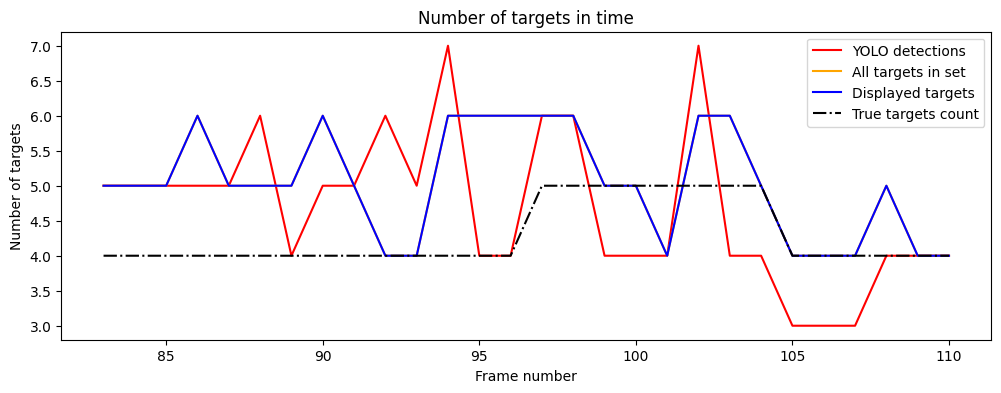
\includegraphics[width=\linewidth]{../../../experiments/E1/V2/YOLO/yolo_det}
    \caption{Development chart of number of detected targets, targets in filter's queue, displayed targets and true targets' count.}
    \label{gr:E1-V2-S1}
\end{figure}

\begin{figure}[H]
    \centering
    \begin{subfigure}{0.48\textwidth}
        \centering
        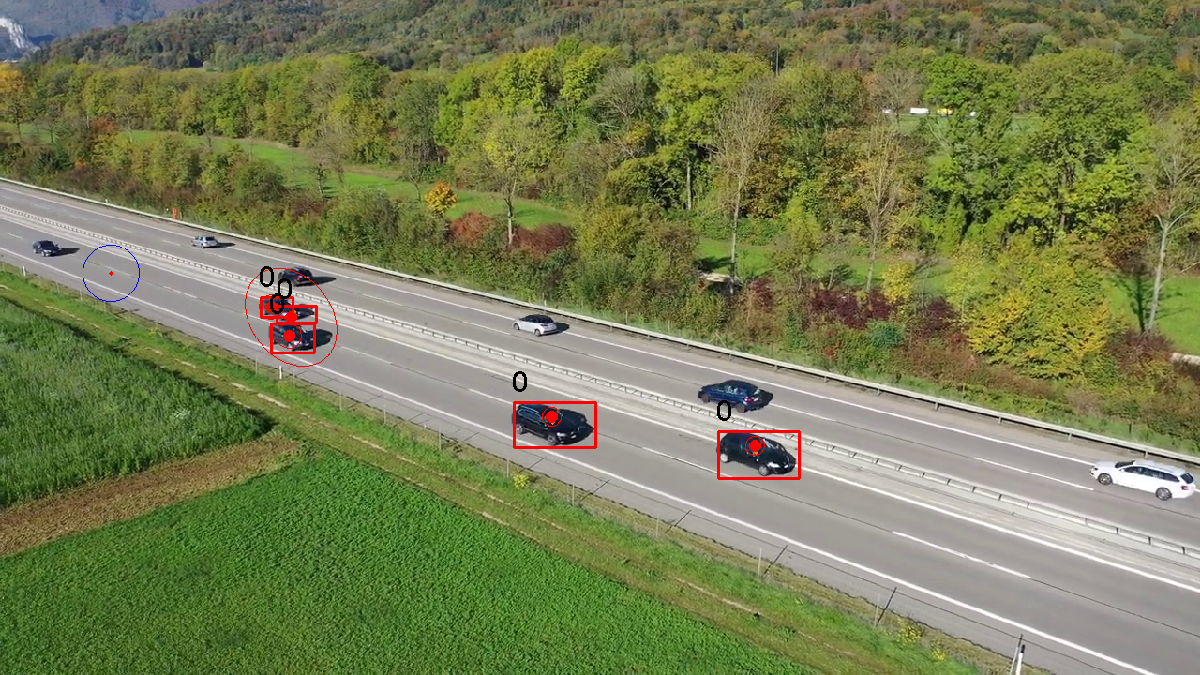
\includegraphics[width=\linewidth]{../../../experiments/E1/V2/YOLO/83}
        \caption{Frame number: 83.}
        \label{fig:E1-V2-S1:01}
    \end{subfigure}
    \begin{subfigure}{0.48\textwidth}
        \centering
        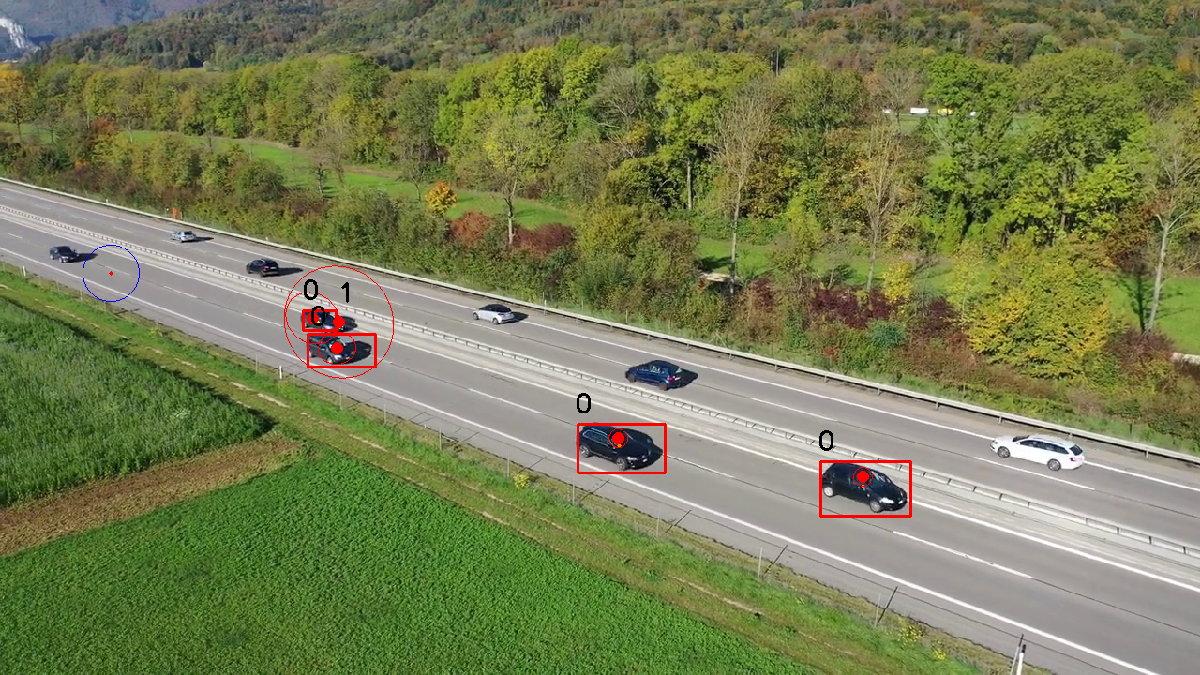
\includegraphics[width=\linewidth]{../../../experiments/E1/V2/YOLO/89}
        \caption{Frame number: 89.}
        \label{fig:E1-V2-S1:02}
    \end{subfigure}
    \\
    \begin{subfigure}{0.48\textwidth}
        \centering
        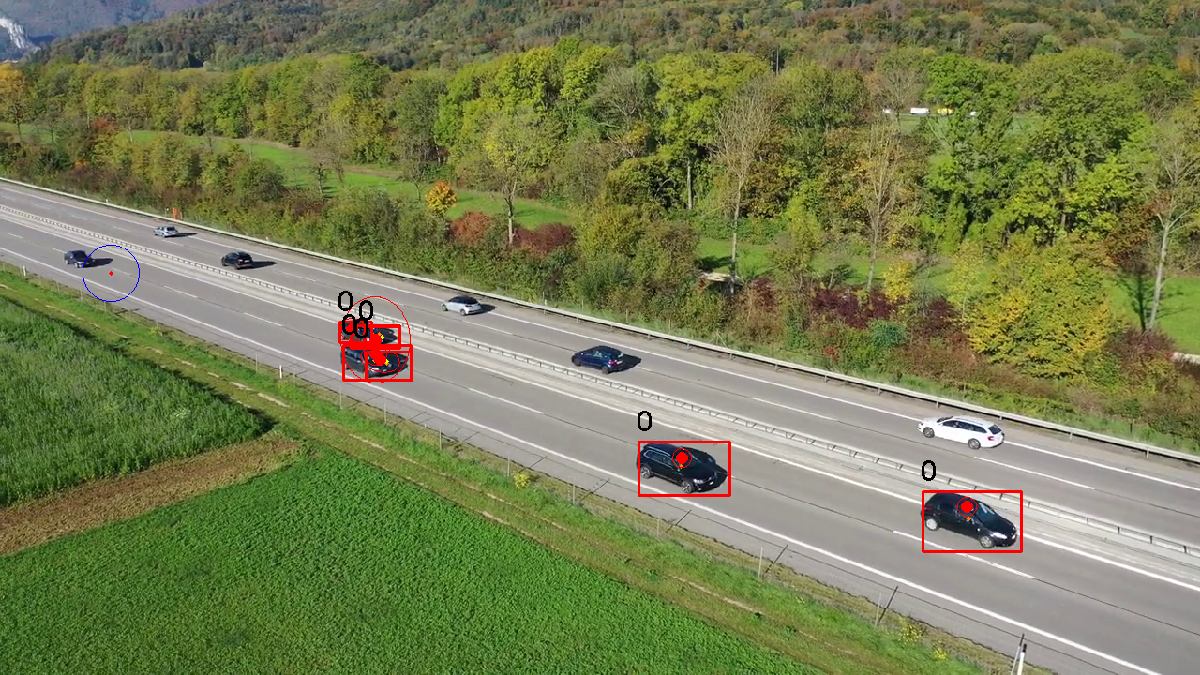
\includegraphics[width=\linewidth]{../../../experiments/E1/V2/YOLO/94}
        \caption{Frame number: 94.}
        \label{fig:E1-V2-S1:03}
    \end{subfigure}
    \begin{subfigure}{0.48\textwidth}
        \centering
        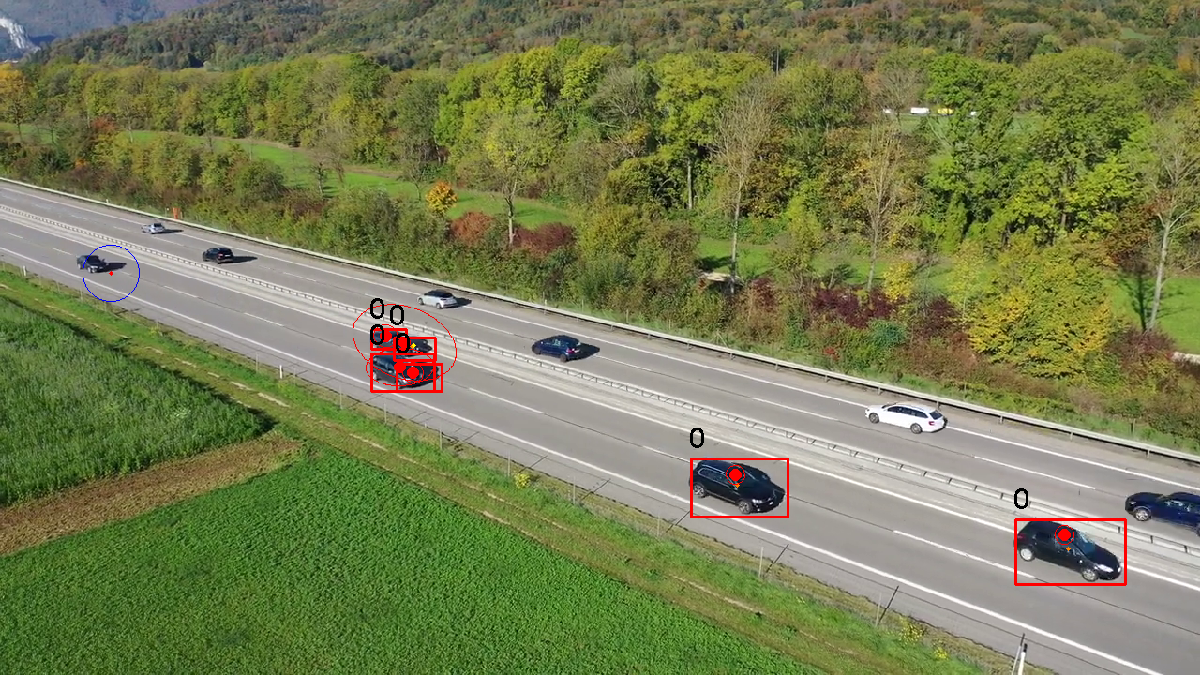
\includegraphics[width=\linewidth]{../../../experiments/E1/V2/YOLO/98}
        \caption{Frame number: 98.}
        \label{fig:E1-V2-S1:04}
    \end{subfigure}
    \\
    \begin{subfigure}{0.48\textwidth}
        \centering
        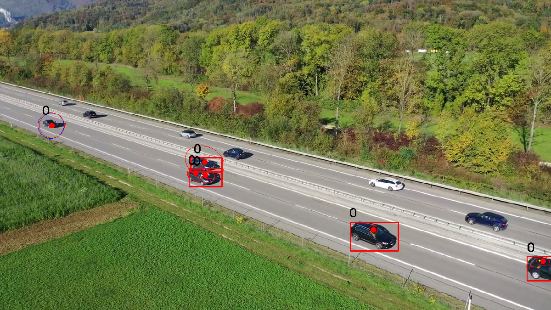
\includegraphics[width=\linewidth]{../../../experiments/E1/V2/YOLO/103}
        \caption{Frame number: 103.}
        \label{fig:E1-V2-S1:05}
    \end{subfigure}
    \begin{subfigure}{0.48\textwidth}
        \centering
        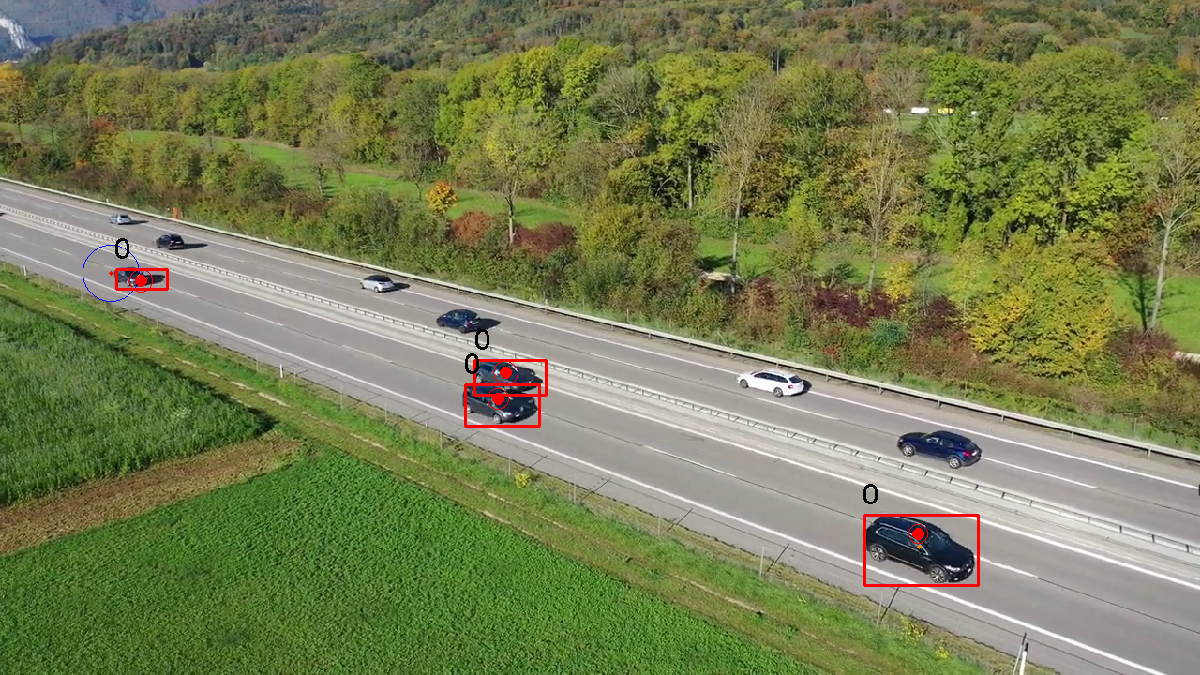
\includegraphics[width=\linewidth]{../../../experiments/E1/V2/YOLO/109}
        \caption{Frame number: 109.}
        \label{fig:E1-V2-S1:06}
    \end{subfigure}
    \caption{Image sequence of tracked objects using GM-PHD filter with dynamic detection probability and YOLO only.}
    \label{fig:E1-V2-S1}
\end{figure}







\subsubsection{S2 -- YOLO + SAM}
As in experiment \textit{E1}, the next settings employs settings \textit{S2} with YOLO object detector and the SAM
segmentation model.
All parameters are included in Table \ref{tab:E1-V2-S2}.
\begin{table}[H]
    \centering
    \begin{tabular}{|c|c|c|c|c|c|c|c|c|}
        \hline
        $P_{D,k}(x)$ & $P$ & $\sigma_{\upsilon}$ & $\sigma_{\epsilon}$ & $T_H$ & $T_d$ & $T_p$ & $T_l$ & $T_{YOLO}$ \\ \noalign{\hrule
        height 1.5pt}
        0.3 & $diag(100,100,100,100)$ & 0.1 & 30 & 1 & 3 & 0.1 & 0.01 & 0.3\\
        \hline
    \end{tabular}
    \caption{The parameter settings for experiment E1-V2-S2 with dynamic detection probability.}
    \label{tab:E1-V2-S2}
\end{table}


The situation resemble the situation with settings \textit{S1}. Four targets occur in Figure \ref{fig:E1-V2-S2:01}.
They continue in they path and all targets are tracked successfully with exception, that there do not appear
additional targets in subsequent frames. The YOLO model detects car's shadow and clasify that as a car, which makes another target in \ref{fig:E1-V2-S2:03}. Due to the merging step, this false target did not survive to the subsequent frames. New car is initialized in \ref{fig:E1-V2-S2:04}. All targets are focused in
last frames.

The number of displayed targets is close to the true number of targets in Graph \ref{gr:E1-V2-S2}. The number of
detected targets exceeds the number of true targets across almost the full line, due to the presence of false
detections.

Settings \textit{S2} perform a little better than settings \textit{S1}, as the number of displayed targets achieves a
smaller error with the true count.

\begin{figure}[H]
    \centering
    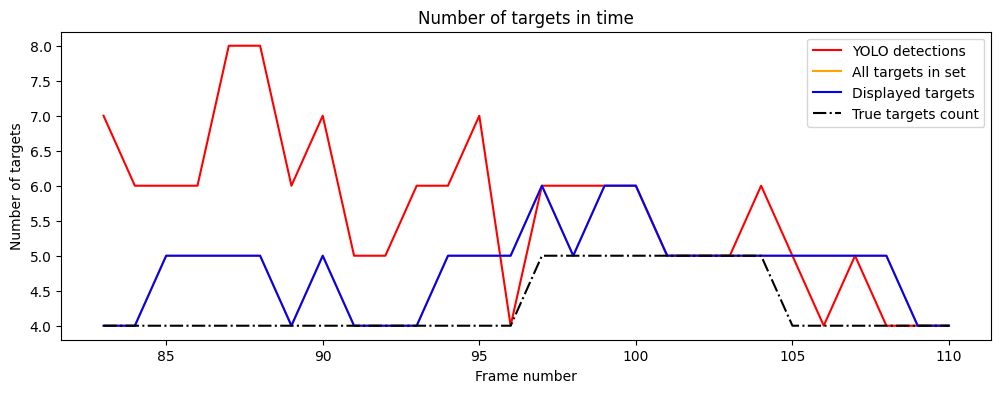
\includegraphics[width=\linewidth]{../../../experiments/E1/V2/SAM/sam_det}
    \caption{Development chart of number of detected targets, targets in filter's queue, displayed targets and true targets' count.}
    \label{gr:E1-V2-S2}
\end{figure}

\begin{figure}[H]
    \centering
    \begin{subfigure}{0.48\textwidth}
        \centering
        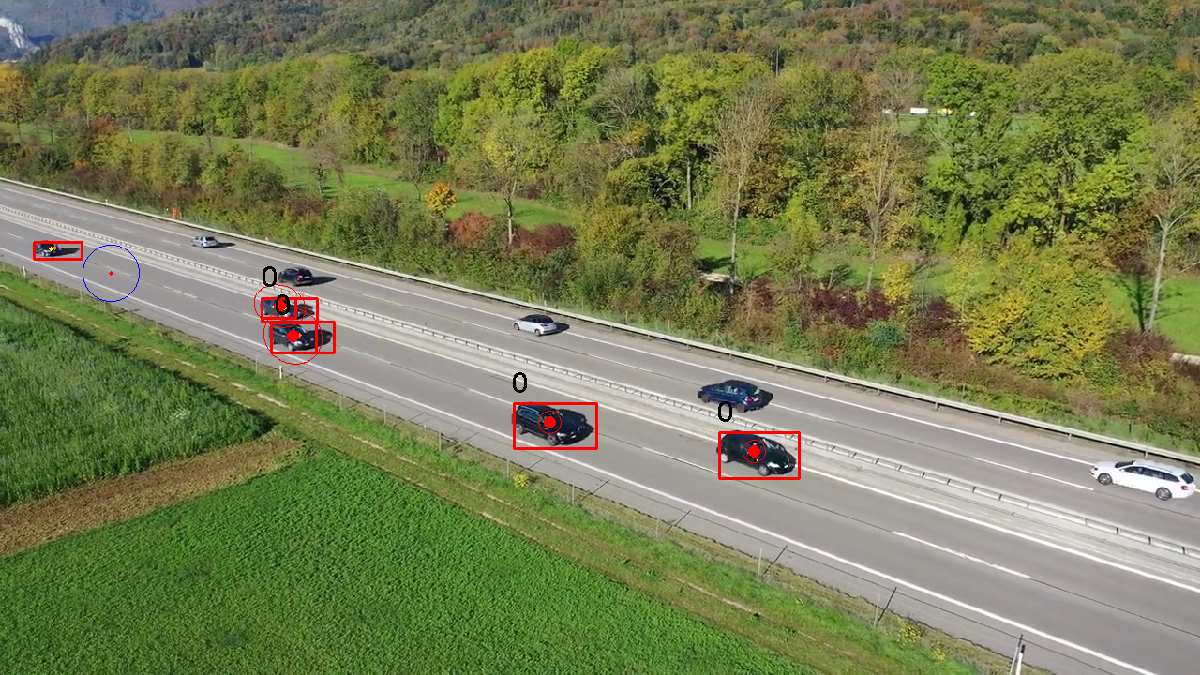
\includegraphics[width=\linewidth]{../../../experiments/E1/V2/SAM/83}
        \caption{Frame number: 83.}
        \label{fig:E1-V2-S2:01}
    \end{subfigure}
    \begin{subfigure}{0.48\textwidth}
        \centering
        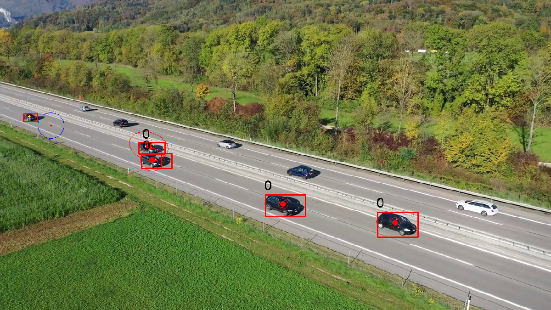
\includegraphics[width=\linewidth]{../../../experiments/E1/V2/SAM/89}
        \caption{Frame number: 89.}
        \label{fig:E1-V2-S2:02}
    \end{subfigure}
    \\
    \begin{subfigure}{0.48\textwidth}
        \centering
        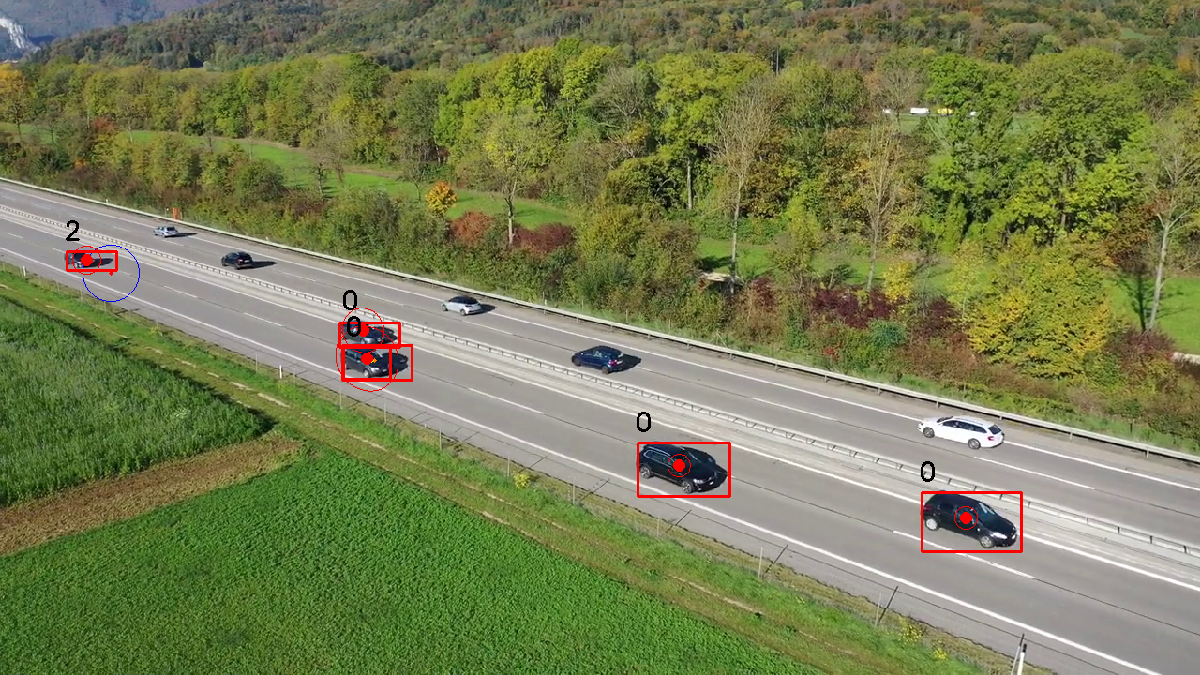
\includegraphics[width=\linewidth]{../../../experiments/E1/V2/SAM/94}
        \caption{Frame number: 94.}
        \label{fig:E1-V2-S2:03}
    \end{subfigure}
    \begin{subfigure}{0.48\textwidth}
        \centering
        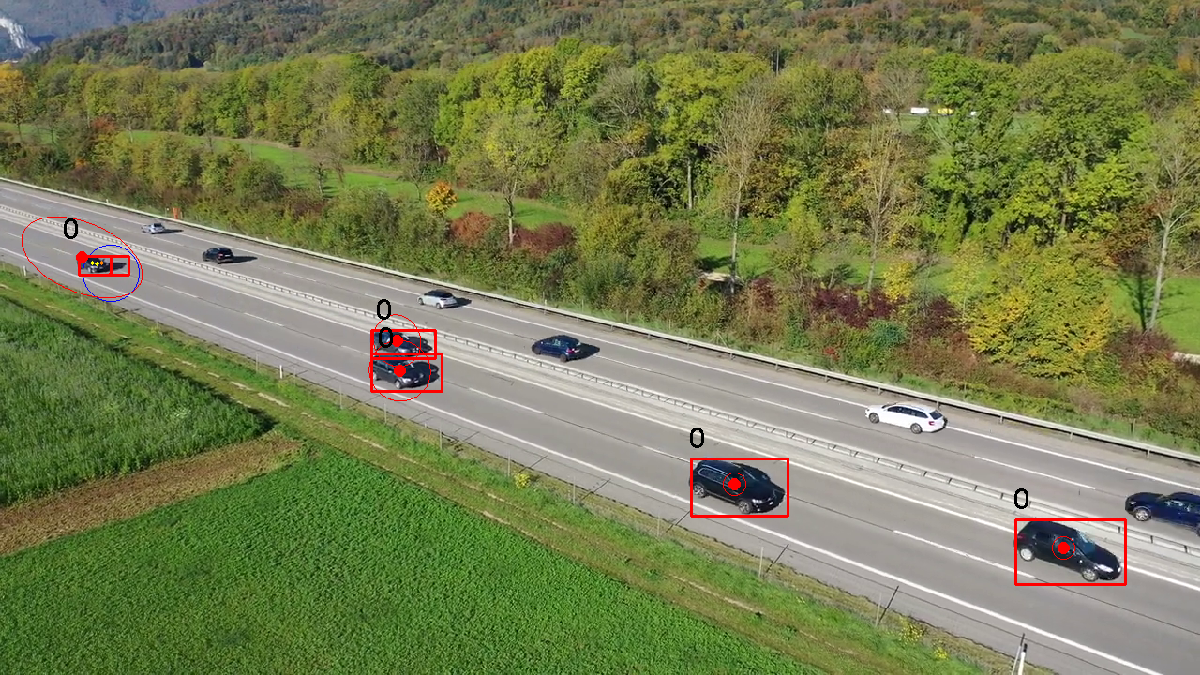
\includegraphics[width=\linewidth]{../../../experiments/E1/V2/SAM/98}
        \caption{Frame number: 98.}
        \label{fig:E1-V2-S2:04}
    \end{subfigure}
    \\
    \begin{subfigure}{0.48\textwidth}
        \centering
        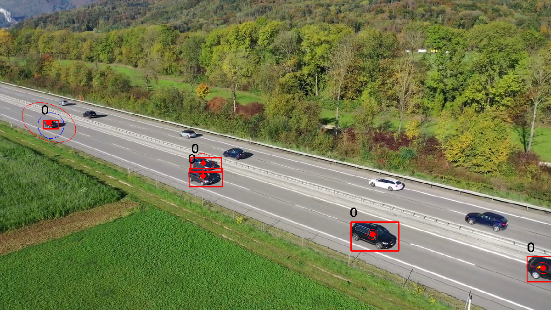
\includegraphics[width=\linewidth]{../../../experiments/E1/V2/SAM/103}
        \caption{Frame number: 103.}
        \label{fig:E1-V2-S2:05}
    \end{subfigure}
    \begin{subfigure}{0.48\textwidth}
        \centering
        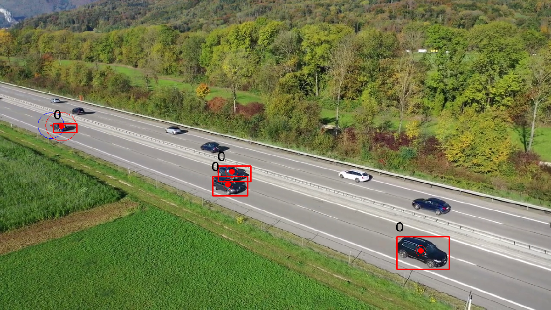
\includegraphics[width=\linewidth]{../../../experiments/E1/V2/SAM/109}
        \caption{Frame number: 109.}
        \label{fig:E1-V2-S2:06}
    \end{subfigure}
    \caption{Image sequence of tracked objects using GM-PHD filter with dynamic detection probability, the YOLO object detector and the SAM image segmentation model.}
    \label{fig:E1-V2-S2}
\end{figure}


\subsubsection{S3 -- Grounded DINO}
The combination of Grounding DINO and SAM is tested on video \textit{V2} as well. Used parameteres are given in Table \ref{tab:E1-V2-S3}.
\begin{table}[H]
    \centering
    \begin{tabular}{|c|c|c|c|c|c|c|c|c|c|}
        \hline
        $P_{D,k}(x)$ & $P$ & $\sigma_{\upsilon}$ & $\sigma_{\epsilon}$ & $T_H$ & $T_d$ & $T_p$ & $T_l$ & $T_{text}$ & $T_{bbox}$\\ \noalign{\hrule
        height 1.5pt}
        0.3 & $diag(100,100,100,100)$ & 0.1 & 30 & 1 & 3 & 0.1 & 0.01 & 0.3 & 0.3\\
        \hline
    \end{tabular}
    \caption{The parameter settings for experiment E1-V2-S3 with dynamic detection probability.}
    \label{tab:E1-V2-S3}
\end{table}

Figure \ref{fig:E1-V2-S3} expos better object detection. As a result, the tracking of objects is more precise than in other settings.
\begin{itemize}
    \item \textbf{\ref{fig:E1-V2-S3:01}:} Starting with four tracked targets in frame no. 83.
    \item \textbf{\ref{fig:E1-V2-S3:02}:} As in experiment E1-V1, the measurement and observation noise covariance seems to be too large for this scenario. The third and fourth car's measurement reaches the validation region of each other. This situation creates new unwanted targets.
    \item \textbf{\ref{fig:E1-V2-S3:03}:} The exact same situation happens in this frame.
    \item \textbf{\ref{fig:E1-V2-S3:04}:} Another car reaches the spawning point.
    \item \textbf{\ref{fig:E1-V2-S3:05}:} Five targets appear in the scene, all of them correctly tracked.
    \item \textbf{\ref{fig:E1-V2-S3:06}:} The scenario ends with four properly detected and tracked objects.
\end{itemize}

Even though two cars driving side by side causes the filter with given parameters modest problems, the merging and pruning step can deal with such situation most of the time, as seen in Graph \ref{gr:E1-V2-S3}. The line showing the number of displayed targets almost copies the line showing the true counts. The graph also shows the problem of two neihbouring targets and the problem of false detections. The peaks in the red line shows these false detections, the filter is able not to be fooled and hold the true number of targets.


As in experiment \textit{E1-V1}, these settings outperforms the other settings. Moreover, due to the more precise object detection, the filter is able to deal with problems like two targets in the same neighbourhood and false detections. However, settings \textit{S3} is very sensitive to measurement and observation noise setting, thus these covariance matrices have to be set carefully.

\begin{figure}[H]
    \centering
    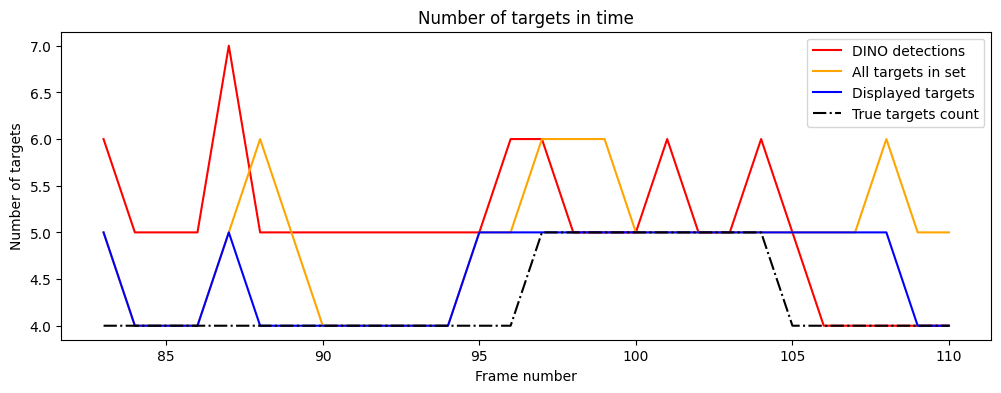
\includegraphics[width=\linewidth]{../../../experiments/E1/V2/DINO/dino_det}
    \caption{Development chart of number of detected targets, targets in filter's queue, displayed targets and true targets' count.}
    \label{gr:E1-V2-S3}
\end{figure}

\begin{figure}[H]
    \centering
    \begin{subfigure}{0.48\textwidth}
        \centering
        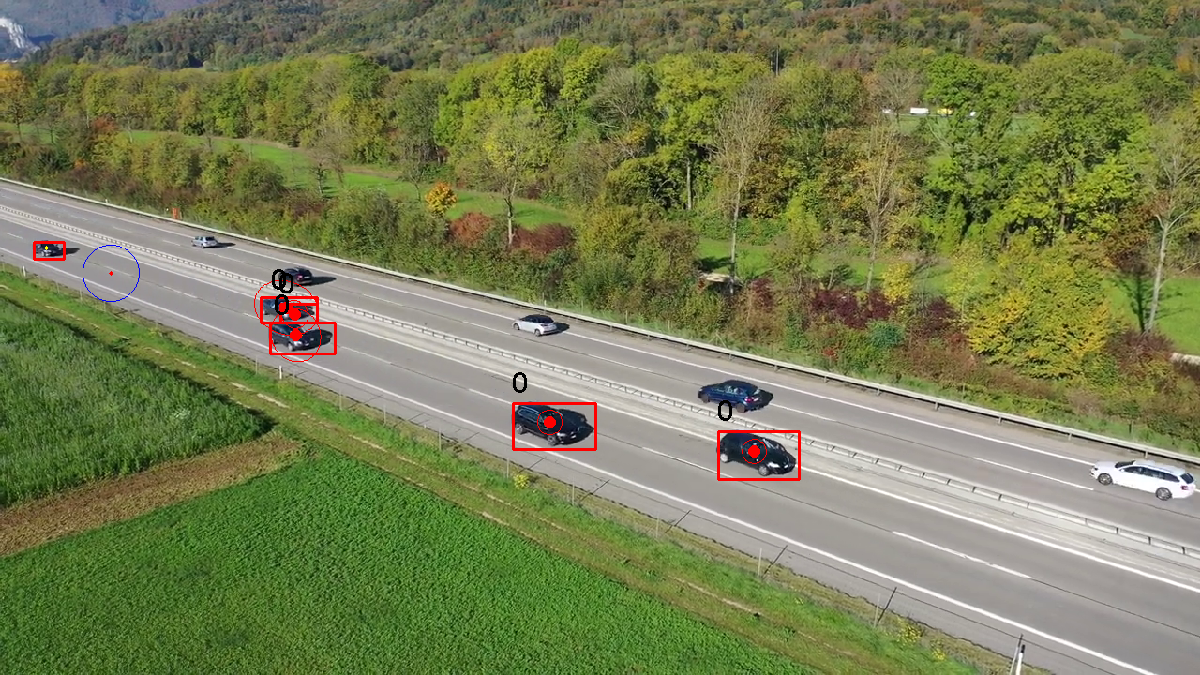
\includegraphics[width=\linewidth]{../../../experiments/E1/V2/DINO/83}
        \caption{Frame number: 83.}
        \label{fig:E1-V2-S3:01}
    \end{subfigure}
    \begin{subfigure}{0.48\textwidth}
        \centering
        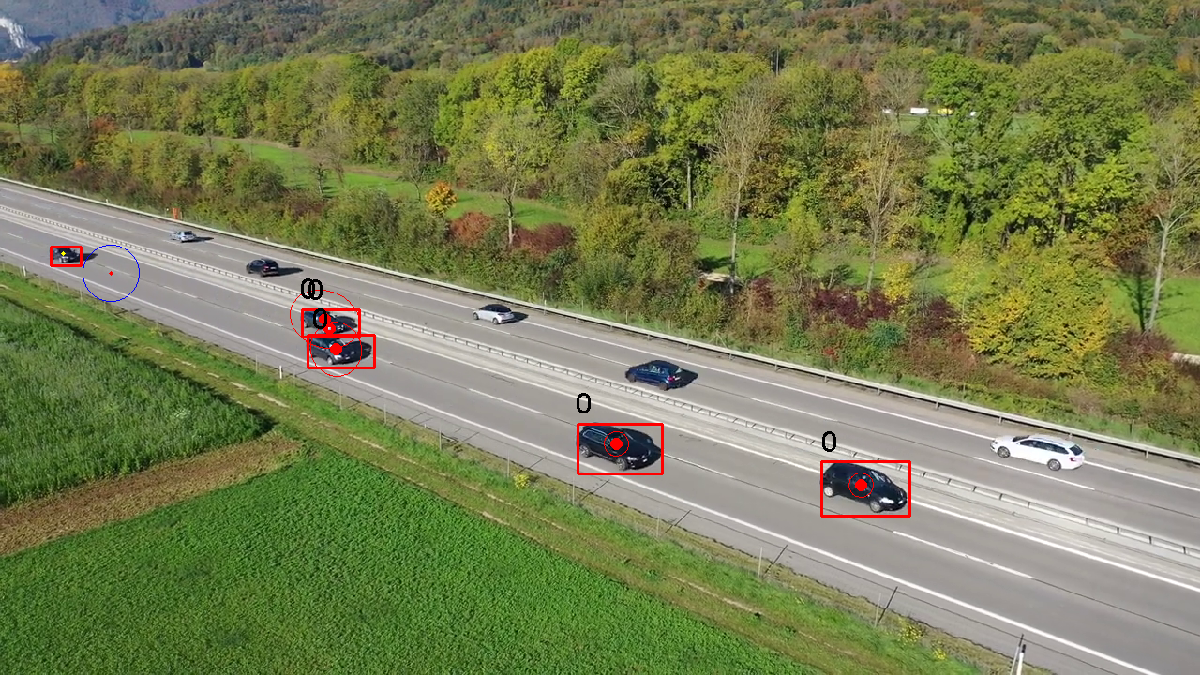
\includegraphics[width=\linewidth]{../../../experiments/E1/V2/DINO/89}
        \caption{Frame number: 89.}
        \label{fig:E1-V2-S3:02}
    \end{subfigure}
    \\
    \begin{subfigure}{0.48\textwidth}
        \centering
        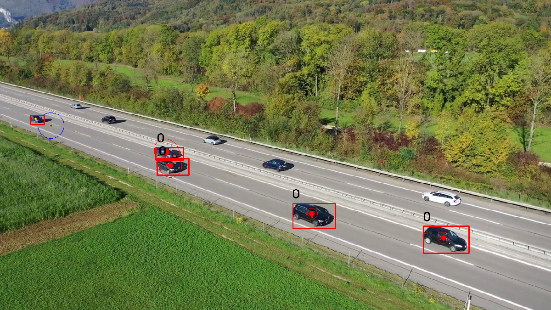
\includegraphics[width=\linewidth]{../../../experiments/E1/V2/DINO/94}
        \caption{Frame number: 94.}
        \label{fig:E1-V2-S3:03}
    \end{subfigure}
    \begin{subfigure}{0.48\textwidth}
        \centering
        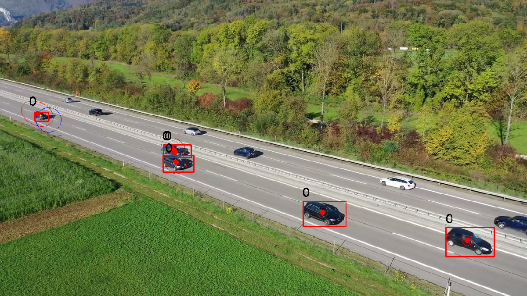
\includegraphics[width=\linewidth]{../../../experiments/E1/V2/DINO/98}
        \caption{Frame number: 98.}
        \label{fig:E1-V2-S3:04}
    \end{subfigure}
    \\
    \begin{subfigure}{0.48\textwidth}
        \centering
        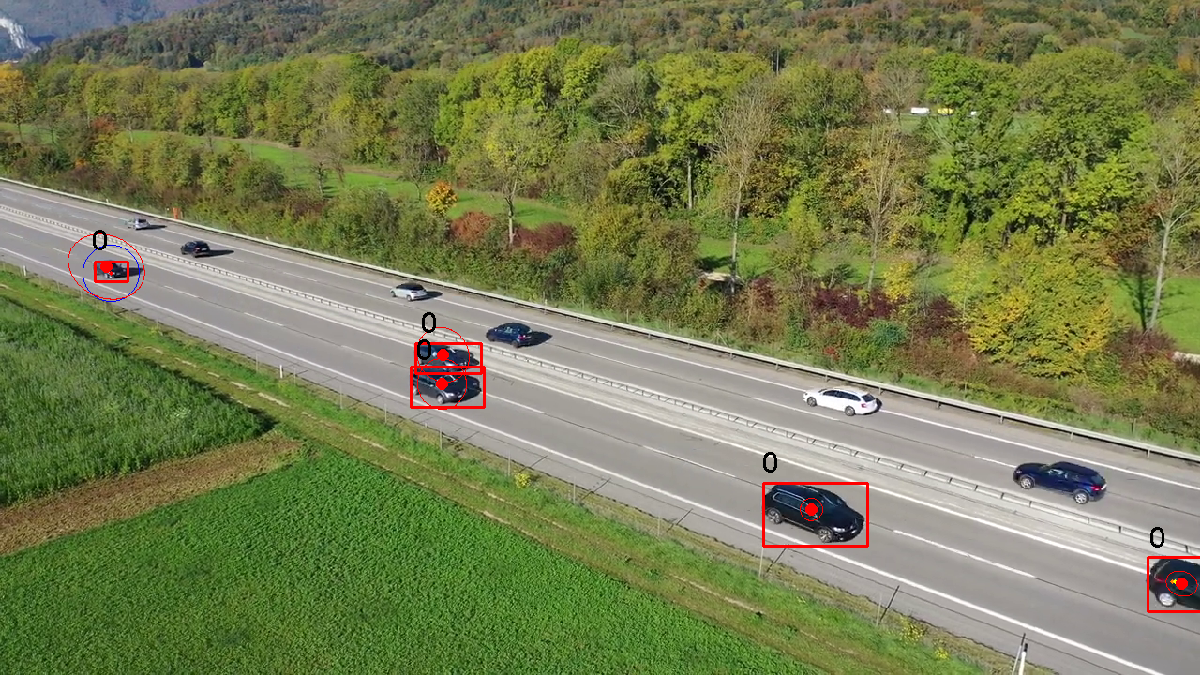
\includegraphics[width=\linewidth]{../../../experiments/E1/V2/DINO/103}
        \caption{Frame number: 103.}
        \label{fig:E1-V2-S3:05}
    \end{subfigure}
    \begin{subfigure}{0.48\textwidth}
        \centering
        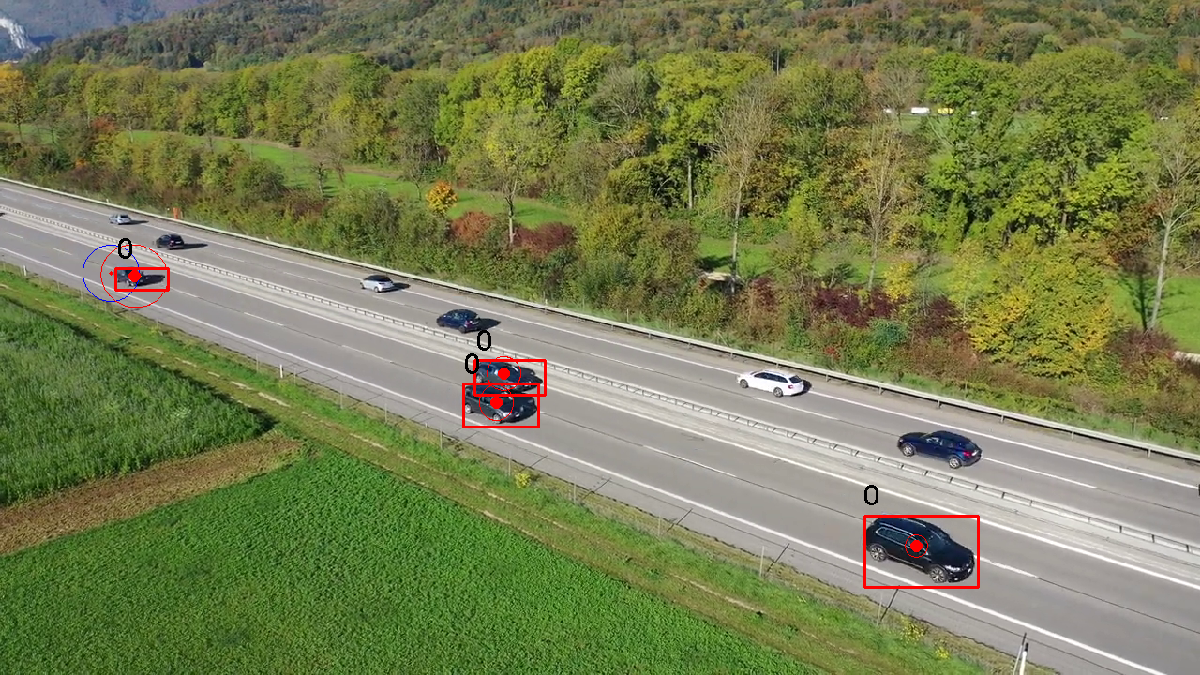
\includegraphics[width=\linewidth]{../../../experiments/E1/V2/DINO/109}
        \caption{Frame number: 109.}
        \label{fig:E1-V2-S3:06}
    \end{subfigure}
    \caption{Image sequence of tracked objects using GM-PHD filter with dynamic detection probability, the DINO object detector and the SAM image segmentation model.}
    \label{fig:E1-V2-S3}
\end{figure}
